The following sections will present the results of our baseline experiments, explore additional ideas for the project, and discuss potential real-world applications.

\subsection{Baseline Experiments}\label{subsec:baseline-results}
\begin{wrapfigure}{r}{0.4\textwidth}
    \centering
    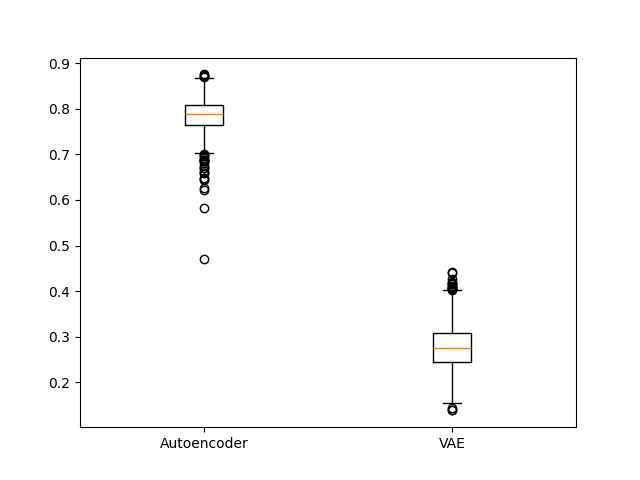
\includegraphics[width=0.4\textwidth]{../../sample_images/evaluation/boxplot_ae_and_vae}
    \vspace{-20pt}
    \caption{Boxplots of per class average SSIM on test data}
    \label{fig:boxplots}
\end{wrapfigure}

We did an exemplary training for 10 epochs on a subset of ImageNet to see if it converges.
The training subset contained 100\,000 images with 100 samples per class, while the test subset contained 10\,000
samples, 10 per class.
We used the PyTorch implementation of the Adam optimizer with a learning rate of 0.001 with a batch size of 128.
This resulted in roughly 780 optimization steps per epoch.
We chose to use 2 latent channels per latent variable using the 32 bit float of pytorch.

\subsubsection{Autoencoder}\label{subsubsec:autoencoder}
When feeding in $3 \times 128 \times 128$ ImageNet images, our latents are of size $\mathbb{R}^{2\times 32 \times 32}$.
From initially $24\text{ bits/pixel}$, the images are compressed down to $4\text{ bits/pixel}$.
We therefore reach a compression rate of 1:6.

We were able to show that our implementation of an \ac{ae} is able to reconstruct images from the ImageNet dataset
passing a first human look.
The average of the SSIM of the test data is $\approx 0.78$ as can be seen in Figure~\ref{fig:boxplots}.

\begin{figure}[H]
    \centering
    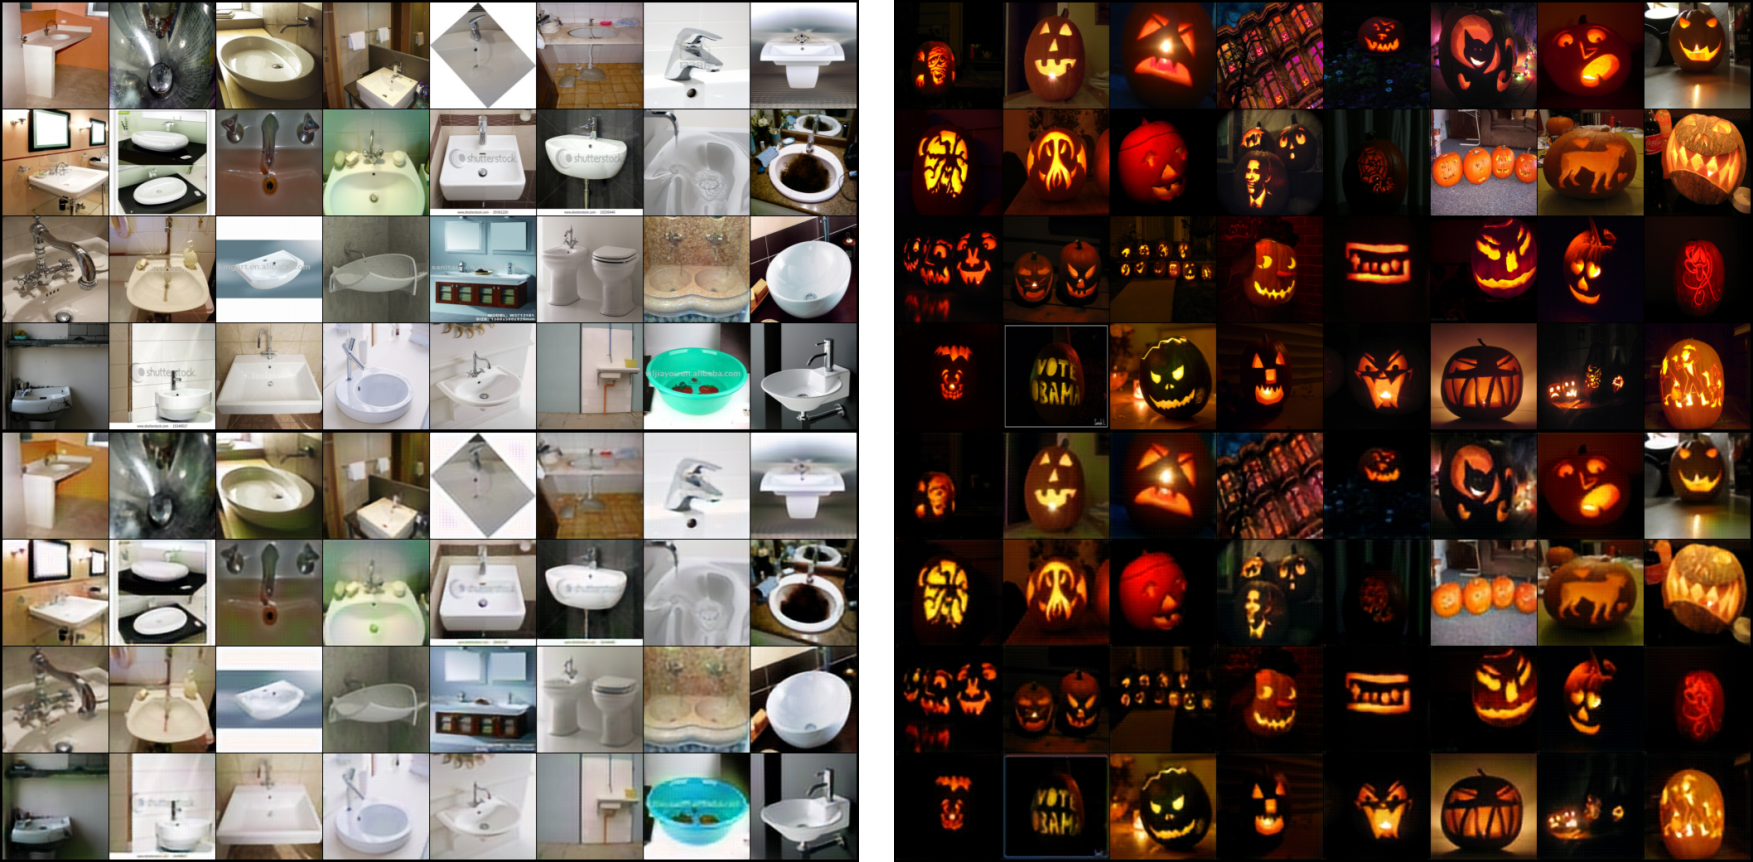
\includegraphics[width=0.6\textwidth]{images/ae_minmax}
    \caption{Best/worst performing class 896/607 of Autoencoder with SSIM of 0.88/0.47}
    \label{fig:imnet_best_perf_ae}
\end{figure}

\subsubsection{VAE}
When using the same latent size as for the \ac{ae}, the \ac{vae} was not able to obtain reconstructions
passing a first visual inspection.
The numeric metrics were also very low, with an average \ac{ssim} below 0.4.
The decoder produced samples that were always very similar, indicating that it may have suffered from posterior
collapse.
When posterior collapse occurs, the learned latent variables fail to encode any meaningful information, effectively
defaulting to the prior distribution.
We plan to revisit our implementation at a later stage and evaluate whether we can enhance it to serve as a more effective baseline.

\begin{figure}[H]
    \centering
    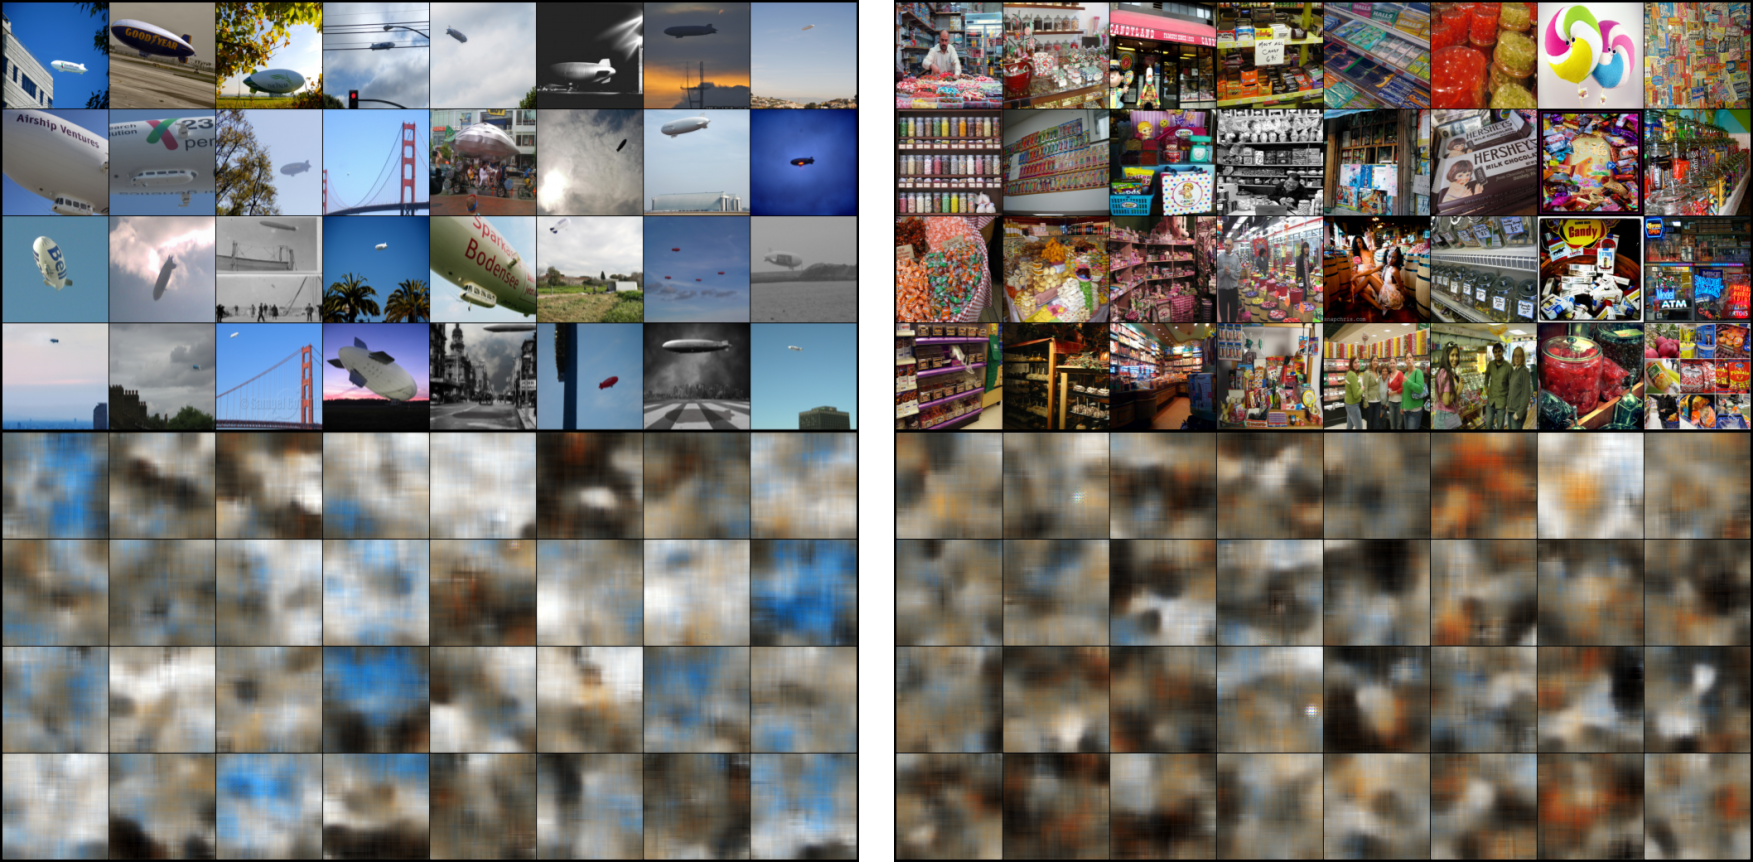
\includegraphics[width=0.6\textwidth]{images/vae_minmax}
    \caption{Best/worst performing class 405/509 of VAE with SSIM 0.44/0.19}
    \label{fig:imnet_best_perf2_vae}
\end{figure}

\subsubsection{JPEG}\label{subsubsec:jpeg}
To compare the compression ability of our baseline methods to JPEG compression, we first had to determine the quality with which JPEG compresses images to approximately 4 bits per pixel.
In a rather small scale experiment, we found that 4 bits per pixel where achieved when using JPEG compression with a quality parameter of 97, which in turn resulted in a \ac{ssim} score of 0.95.
This shows that neural image compression using the baseline methods are outperformed by JPEG compression.

\subsection{Further inspection}
We further inspected the performance of our models on a per class basis. Figure \ref{fig:boxplots} shows the distribution of SSIM of the images of each class for both VAE and Autoencoder. \ac{vae} performs worse in all classes. The \ac{ae} is on average better than the \ac{vae} on the test data, though there are performance differences between class. 

\ac{ae} performs significantly worse on some classes.
The lowest SSIM score is 0.47 for class \textit{jack-o'-lantern}, though there is
hard to see any difference between that class images and those of the best performing class
\textit{washbasin} (0.88 SSIM)~\ref{fig:imnet_best_perf_ae}.
This discrepancy may be explained by the findings of ~\cite{understandingssim}, which show that SSIM lacks
comparability in dark regions. The images from the \textit{jack-o'-lantern} class are notably dark, which could contribute to this issue.

It is surprising that the best-reconstructed images by the \ac{vae}, with an SSIM of 0.44, are significantly worse than the worst-reconstructed images by the \ac{ae}, despite having a very similar SSIM.

\subsection{Dataset}\label{subsec:dataset}
We discuss the relevance of the dataset to real-world applications and its suitability for our task.
\subsubsection{Real-world Application}
CIFAR-10 and ImageNet have been foundational datasets for over a decade and a half.
Their primary use-case has shifted from being cutting-edge datasets for training state-of-the-art models like the
work from~\cite{AlexNet}, to serving as a base for experiments and benchmarks.

Nowadays, state-of-the-art generative models rely on much larger datasets, often containing billions of samples.
A notable example is LAION-5B~\cite{laion5b} which was used to train the Stable Diffusion model introduced by~
\cite{stable_diff}.

Throughout the same paper, ImageNets continuing relevancy can be observed, as it is used to train and evaluate
experimental models.
Its still substantial capacity allows for the generalization of good performance to larger and more diverse datasets.
Additionally, inception based metrics like \ac{fid} are also calculated using ImageNet.

Similar trends can be observed with CIFAR-10; however, its low resolution restricts its applicability for
benchmarking contemporary image generation approaches.

\subsubsection{Suitability}
While we still intend to work with CIFAR-10 for comparison and fast prototyping, its lower capacity makes it less
promising to us.

Despite the assessment that ImageNet is comparably smaller than datasets employed for current large-scale
models, it remains a big and diverse dataset.
This represents both the greatest advantage and the greatest challenge of this dataset for us.

The challenge lies in the heterogeneous shapes and properties of individual classes and their distributions.
Additionally, its vast size necessitates a heavy reliance on statistical analysis, as manually inspecting samples has
only limited feasibility at this scale.

On the other hand, the size and diversity of the data is of course a huge advantage for training the models.
The models will be able to learn a wide range of features and patterns, and to generalize it to unseen data.

The results from our initial training runs, using only a small subset of the training data, demonstrate promising
outcomes.
The model has neither converged yet on test nor the training data.
We therefore anticipate potential for further improvement by training the model on the full dataset until
convergence, which could enhance its performance.

Sampling functionality has not yet been implemented; however, due to its still wide-spread use for experimental
models we expect that the dataset is sufficient for training our generative models.
Especially due to its comparably lower size to modern datasets, we do not anticipate achieving the level of visual
fidelity demonstrated by state-of-the-art techniques.

\subsection{A prospect on further Experiments}\label{subsec:further-ideas}
To ensure comparability with the paper, we use \ac{mse} loss for training our \ac{ae}, even though, as discussed in~\ref{subsec:compression}, this may not be the most optimal metric for aligning with human perception.
\ac{ssim} is a metric for precisely this purpose, so we think our models might benefit from using it as a loss
function instead of \ac{mse}.
In ~\cite{ssim_as_loss}, it is shown that using a loss function targeted to human perception can improve the quality
of convolutional neural networks for image reconstruction, in particular using \ac{ssim}.

\subsection{Outlook: Why the \ac{vq}?}\label{subsec:final-words}
Image reconstruction as well as image generation are two relatively well researched and active topics.
The \ac{vae} is a classical approach to this field.
\ac{vae} can sample in the latent space and generate new images by virtue of their stochastic properties.

But a discrete latent is sometimes favored over latent distributions, because of their simplicity, interpretability
and compatibility with other modalities ~\cite{vqvae}.
They also represent the inherent discrete nature of image datasets best.
The \ac{vae} model is also limited by the problem of posterior collapse, which we likely experienced throughout our
experiments.

Over the next milestones, we will try to verify, that the \ac{vq} architecture can fill that gap, and combine the
favorable properties of the \ac{vae} with a discrete latent space.